\chapter{Introduction to Artificial Neural Networks}
\chapterintrobox{Artificial neural networks are computational systems capable of finding complex functions that link an input to an output. These systems can be used for a variety of tasks such as regression and classification. They can be used in predictive maintenance and prognostics to estimate the health of equipment and predict with some uncertainty its remaining useful life. This chapter discusses neural networks, their topology, training and mathematical formulation.}

\section{Structure of artificial neural networks}
Artificial neural networks are computational systems used to find the mapping between an input and an output, they consist of several layers (input layer, output layer and an arbitrary number of hidden layers between the input and the output) and each layer contains a number of neurons where each neuron in each layer is connected to all neurons in the previous and the next layer (except for the input and output layers which are connected only to the next and the previous layer respectively).
Each neuron of each layer receives an input from the neurons of the previous layer (in the form of a vector), multiplies the vector by a few weights and sums the result and then applies a linear activation function. Each neuron ends up with a single numerical value called activation, which will be passed on to the neurons in the next layer.

Figure \ref{fig:neural-network-structure} shows a neural network with the following structure:

\begin{itemize}
    \item Input layer with 3 inputs
    \item Single hidden layer with 4 neurons
    \item Output layer with 1 neuron
\end{itemize}

\begin{figure}[h]
    \centering
	

	
		
		
\begin{tikzpicture}[neuron/.style={circle,draw, thick,align=center, minimum size=2em,inner sep=1pt}, input/.style={->}]

\node[text width=2cm, align=center] at (0,.5*\nodedist) {\small Input Layer};

\node[text width=2cm, align=center] at (\layerdist,.5*\nodedist) {\small Hidden Layer};

\node[text width=2cm, align=center] at (2*\layerdist,.5*\nodedist) {\small Output Layer};

\foreach \y in {1,...,3} \node[] (in\y) at (-\layerdist*.5,-\y*\nodedist) {$x_\y^{(i)}$};  

\foreach \y in {1,...,3} \node[neuron]  (I\y) at (0,-\y*\nodedist) {$a_\y^{[1]}$};  

\foreach \in in {1,...,3} \draw[->, >=angle 60] (in\in) --  (I\in);

\foreach \y in {1,...,4} \node[neuron]  (H\y) at ($(\layerdist,-\y*\nodedist) +(0, .5*\nodedist)$) {$a_\y^{[2]}$};

\foreach \y in {1,...,1} \node[neuron] (O\y) at ($(I2) + (2*\layerdist, 0)$) {$a_\y^{[3]}$};

\node at ($(I2) + (2.5*\layerdist, 0)$) (y) {$\hat{y}^{(i)}$};


\foreach \dest in {1,...,4} \foreach \source in {1,...,3} \draw[->, >=angle 60] (I\source) -- (H\dest);

\foreach \dest in {1,...,1} \foreach \source in {1,...,4} \draw[->, >=angle 60] (H\source) -- (O\dest);

\draw[->, >=angle 60] (O1) -- (y);

\draw[->,  thick, >=angle 60] (.5*\layerdist,-4.5*\nodedist) -- node[above] {Direction of forward propagation} (1.5*\layerdist,-4.5*\nodedist);
\draw[->,  thick, >=angle 60]  (1.5*\layerdist,-4.8*\nodedist)-- node[below] {Direction of backpropagation} (.5*\layerdist,-4.8*\nodedist);
\node [anchor=west] (note) at (-1.3*\layerdist,-4*\nodedist) {\footnotesize Single neuron};
\draw [->,  thick, >=angle 60] (note) to[out=0, in=-120] (I3.south);
\end{tikzpicture}
		
		

    \caption{Structure of an artificial neural network}
    \label{fig:neural-network-structure}
\end{figure}

\section{Feedforwad networks: from input to output}
\label{section:feedforward-neural-network}
The architecture of figure \ref{fig:neural-network-structure} is called Feedforward Neural Network, it is an acyclic architecture where information flows from the first to the last layer without any internal loop, unlike other architectures such as recurrent neural networks. The first layer is the input layer, it does not perform any operation and is limited to receiving input. The input is a vector of numbers representing the different variables. The vector is multiplied by a matrix of weights that transforms it and sends it to the next layer (or to the first hidden layer). An activation function is applied to the values resulting from the multiplication of the values of the previous layer with the weight matrix, the result becomes the values of the next layer, or activations (the value of each neuron is called activation).

A general formula for moving from the $l-1$ layer to the $l$ layer is given by the equation \ref{equation:forward-step}:

\begin{equation}
    a^{[l]} = g^{[l]}(W^{[l]}a^{[l-1]}+b^{[l]})
    \label{equation:forward-step}
\end{equation}

Where $g^{[l]}$ is the activation function of the $l$ layer, $W^{[l]}$ is the weights matrix that transforms the values (activations) from the $l-1$ layer to the $l$ layer and $a^{[l]}$ represents the activations of the $l$ layer. $b$ is the value of the bias (or intercept value), it is added to the multiplication between the activations and the weights matrix, it is a parameter that can be learned like the weights. The operation is repeated for each layer up to the output layer.
The first layer can be considered as layer 0 and the inputs can be designated by the vector $a^{[0]}$.

\section{Activation functions}
The activation functions are applied to the result of multiplying the inputs of the previous layer with the corresponding weights to determine the value of each neuron. There are different types of these functions.

The use of the non-linear activation function is very important for neural networks, they allow learning the complex non-linear mapping from input to output. If the network does not use non-linear activation (for example, linear activation or the identity function), then the whole network (regardless of its depth) is equivalent to a network with only one hidden layer.

There are a variety of activation functions that can be used for the hidden and output layers. Figure \ref{fig:activation-function} shows some examples:
\begin{figure}[h]
    \centering
	\documentclass[12pt]{article}
\usepackage[margin=1in]{geometry}
\usepackage{tikz}
\usetikzlibrary{arrows}
\usepackage{pgfplots}

\usepackage{caption}
\usepackage{subcaption}
\begin{document}



\begin{figure}
\begin{subfigure}[b]{0.24\linewidth}


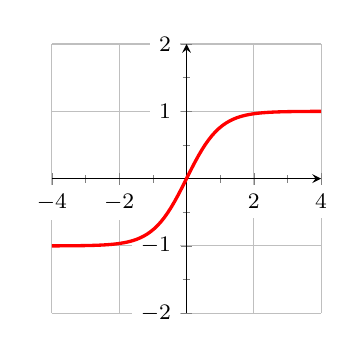
\begin{tikzpicture}
	\begin{axis}[ 
%title=$\tanh(x)$,
xmin=-4, xmax=4,ymin=-2, 
ymax=2, grid=major,
height=5cm, width=5cm,
axis line style={latex-latex},
axis lines=middle,
ticklabel style={font=\footnotesize,fill=white},
minor tick num=1,
scaled ticks=false] 
\addplot[samples=100,red,very thick] {tanh(x))};
%\addlegendentry{$\tanh(x)$}
\end{axis}
\end{tikzpicture} 
\subcaption{tanh}
\end{subfigure}
\hfill
\begin{subfigure}[b]{0.24\linewidth}



	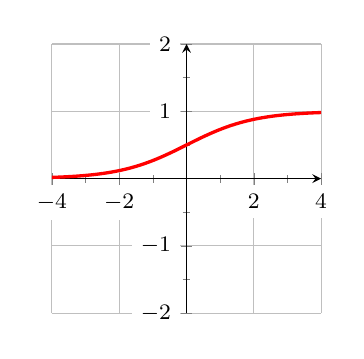
\begin{tikzpicture}
	\begin{axis}[ 
	%title=$\tanh(x)$,
	xmin=-4, xmax=4,ymin=-2, 
	ymax=2, grid=major,
	height=5cm, width=5cm,
	axis line style={latex-latex},
	axis lines=middle,
	ticklabel style={font=\footnotesize,fill=white},
	minor tick num=1,
	scaled ticks=false] 
	\addplot[samples=100,red,very thick] {1/(1+exp(-x))};
	%\addlegendentry{$\tanh(x)$}
	\end{axis}
	\end{tikzpicture}
	
	
	
\subcaption{sigmoid}
\end{subfigure}
\hfill
	\begin{subfigure}[b]{0.24\linewidth}
		
		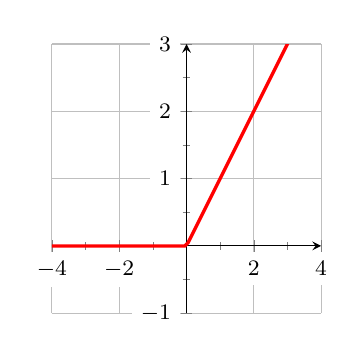
\begin{tikzpicture}
		\begin{axis}[ 
		%title=$\tanh(x)$,
		xmin=-4, xmax=4,ymin=-1, 
		ymax=3, grid=major,
		height=5cm, width=5cm,
		axis line style={latex-latex},
		axis lines=middle,
		ticklabel style={font=\footnotesize,fill=white},
		minor tick num=1,
		scaled ticks=false] 
		\addplot[samples=100,red,very thick] {max(0,x)};
		%\addlegendentry{$\tanh(x)$}
		\end{axis}
		
		\end{tikzpicture}

\subcaption{ReLU}
	\end{subfigure}
\hfill
		\begin{subfigure}[b]{0.24\linewidth}
			
		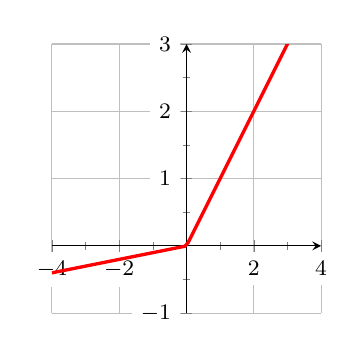
\begin{tikzpicture}
		\begin{axis}[ 
		%title=$\tanh(x)$,
		xmin=-4, xmax=4,ymin=-1, 
		ymax=3, grid=major,
		height=5cm, width=5cm,
		axis line style={latex-latex},
		axis lines=middle,
		ticklabel style={font=\footnotesize,fill=white},
		, xticklabel style={anchor=north},
		minor tick num=1,
		scaled ticks=false] 
		\addplot[samples=100,red,very thick] {max(0,x)+min(0,0.1*x)};
		%\addlegendentry{$\tanh(x)$}
		\end{axis}
		
		\end{tikzpicture}
		\subcaption{Leaky ReLU}
		\end{subfigure}
			
			\caption{Different activation functions}	

\end{figure}
\end{document}
    \caption{Different activation functions}
    \label{fig:activation-function}
\end{figure}

Table \ref{table:activation-functions} shows mathematical definition of several activation functions:

\begin{table}[h]
    \centering
    \begin{tabular}{c|c}
        \hline
        Activation function & Mathematical definition \\
        \hline
        Identity (no activation) & Id(x) = x \\
        Sigmoid & $\sigma(x)= \frac{1}{1+e^{-x}}$ \\
        tanh & $tanh(x)=\frac{(e^x-e^{-x})}{(e^x+e^{-x})}$\\
        Rectified Linear Unit (ReLU) & $ReLU(x)=max(0,x)$\\
        Leaky ReLU & $LeakyReLU(x)=max(0.1 x,x)$\\
    \hline
        
    \end{tabular}
    \caption{Mathematical definition of several activation functions}
    \label{table:activation-functions}
\end{table}


\section{Network training}
The process of training a neural network consists of determining the weights (coefficients) that map the neurons of each layer to the neurons of the next layer. This process can be formulated in more mathematical terms as an optimization problem: optimization of the network coefficients to find their values that minimize a cost function.

Neural network training uses training data that provide inputs and their corresponding outputs.

\subsection{Cost function}
The cost function is the function used to calculate the difference between the output of the neural network and the expected actual output, it quantifies the performance of the network. The goal of the training process is to minimize this function by using Gradient Descent (see next section) to find the best set of weights that gives the lowest difference between the training data and the network prediction.

There are many types of cost functions, each type corresponds to different neural networks tasks (e.g. regression, binary classification, …). The cost function usually used for regression problems is mean-squared error function (Equation \ref{equation:mse}) which calculates the sum of distances between the model predictions $\hat{y}_i$ and the actual output ($y_i$), $N$ is the number of data points available for training:
\begin{equation}
    MSE=\frac{1}{N}\sum_{i=1}^N(y_i-\hat{y}_i)
    \label{equation:mse}
\end{equation}

The other major task of neural networks and other types of models is classification. There are two main types of classification: binary classification, or classification of two classes and multiclass classification or classification of many classes. The first one uses binary cross-entropy loss function (Equation \ref{equation:logloss}) and the latter uses categorical cross-entropy.

\begin{equation}
    BCE = \sum_{i=1}^{N}\hat{y}_i log(y_i)+(1-\hat{y}_i)log(1-\hat{y}_i)
    \label{equation:logloss}
\end{equation}

The choice of activation function for the last layer of the network is directly related to the used cost function. For regression tasks, linear activation function is used. For binary classification it's sigmoid and for multiclass classification it's softmax function.

\subsection{Gradient Descent}
Gradient Descent is an iterative optimization algorithm used to optimize a differentiable function. Gradient Descent works by calculating the gradients of the objective function and then taking iterative steps in the negative direction of the gradients.

\subsection{Convex and non-convex functions}
Gradient descent in neural networks is used to optimize (minimize) the cost function by finding the best set of weights and biases that give the lowest cost possible. Objective functions can be categorized into two types: convex and non-convex functions.
A convex function is said to be convex if it has the property that every chord lies on or above the function. Any value of $x$ in the interval from $x=a$ to $x=b$ can be written in the form $\lambda a+(1-\lambda)b$ where $0\leq\lambda\leq 1$. The corresponding point on the chord is given by $\lambda f(a)+(1-\lambda)f(b)$, and the corresponding value of the function is $f(\lambda a+(1-\lambda)b)$ (Figure \ref{fig:convexity}). Convexity then implies:
\begin{equation}
    f(\lambda a+(1-\lambda)b)\leq \lambda f(a)+(1-\lambda)f(b)
    \label{equation:convexity}
\end{equation}

This is equivalent to the requirement that the second derivative of the function be everywhere positive \cite{Bishop2006}. This condition of convexity can be extended to spaces with arbitrarily large number of dimensions.

\begin{figure}[h]
    \centering
    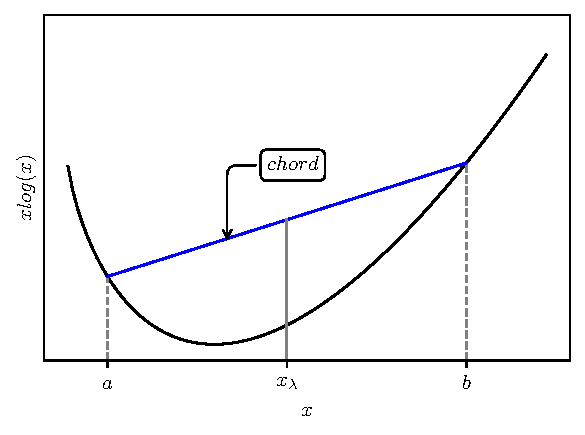
\includegraphics{figures/convex_function.pdf}
    \caption{Condition of convexity}
    \label{fig:convexity}
\end{figure}

A non-convex function is a function that doesn't satisfy the convexity condition. Figure \ref{fig:convex-nonconvex-functions} shows an example of a convex (left) and a non-convex function (right) where the function parameters are in two-dimensional space.

\begin{figure}[h]
    \centering
    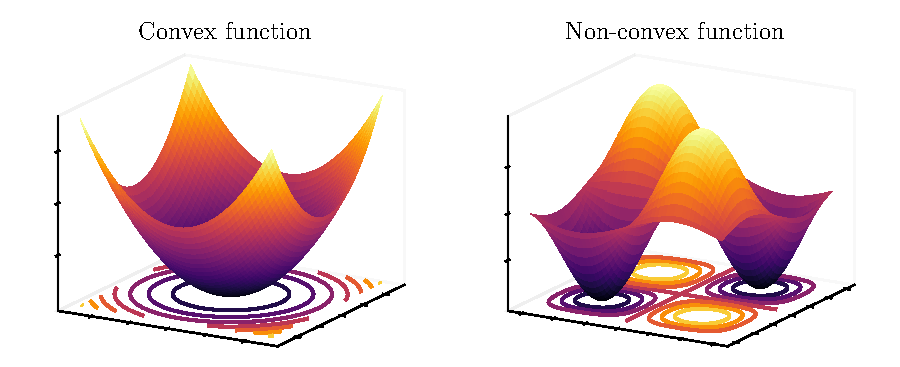
\includegraphics{figures/gradient_descent.pdf}
    \caption{Example of convex and non-convex functions}
    \label{fig:convex-nonconvex-functions}
\end{figure}

\subsection{Global and local minima}
Global minimum refers to the lowest possible value in a set (or of a function). Finding the global minimum refers to finding the set of parameters that correspond to this minimum value. When the function is convex, finding the global maximum is possible and easy, algorithms like gradient descent always converge to the global minimum in convex optimization. Examples of convex cost functions is linear regression cost function. For more complex models such as neural networks, cost function is highly non-convex with many local minima.

Figure \ref{fig:global_local_minima} shows an example of a non-convex function with a global and local minima. The problem with non-convex optimization is that the optimization algorithm can converge to the local minimum instead of the global one. The algorithm convergence is related to the random initialization of network weights.

\begin{figure}[h]
    \centering
    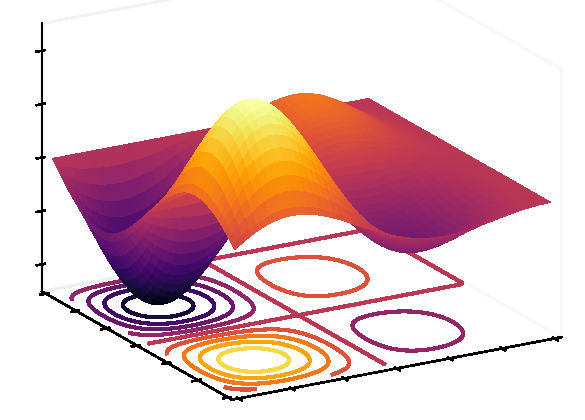
\includegraphics{figures/global_local_minima.pdf}
    \caption{Non-convex function with global and local minima}
    \label{fig:global_local_minima}
\end{figure}

\subsection{Saddle points}
A saddle point or minimax point is a point on the surface of the graph of a function where the slopes (derivatives) in orthogonal directions are all zero (a critical point), but which is not a local extremum of the function (Figure \ref{fig:saddle-point}).

\begin{figure}[h]
    \centering
    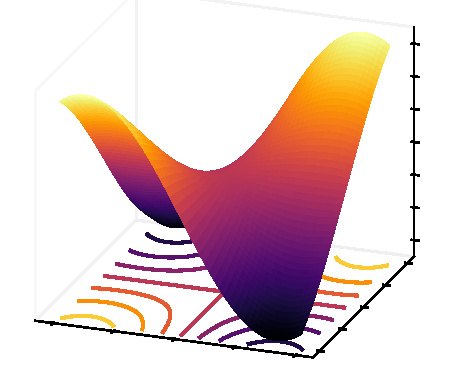
\includegraphics{figures/saddle_point.pdf}
    \caption{Saddle point}
    \label{fig:saddle-point}
\end{figure}

\subsection{Optimization of multilayer networks}
In  \cite{Choromanska2014} the authors showed that getting stuck in poor local minima is a major problem only for shallow networks but becomes gradually of less importance as the network size increases. This is mainly due to the fact that in large networks, local minima lie close to the global minimum so they yield similar good performance.

The following hypotheses were also verified empirically in the mentioned paper regarding learning with large-size networks:
\begin{itemize}
    \item When a network is large, there isn't a significant difference in performance on test data among most of local minima.
    \item Probability of finding a bad local minimum in small networks is higher than the probability of finding them in larger networks.
    \item Finding the global minimum on training set doesn't guarantee a better performance on testing data, rather it could cause overfitting and reduced performance.
\end{itemize}

\subsection{Backpropagation}
Backpropagation is the algorithm used to calculate the gradients of the cost function (the objective function) of a neural network. Since a neural network can be interpreted as functions composition, Backpropagation uses the derivation theorem of a composition of functions to find the gradients in relation to the network weights.

The use of Backpropagation for training neural networks was popularized by David E. Rumelhart, Geoffrey E. Hinton and Ronald J. Williams \cite{Rumelhart1986}, they described it as a procedure that repeatedly adjusts the weights of the network connections so as to minimize a measure of the difference between the actual output vector of the network and the desired output vector. As a result of the weight adjustments, "hidden" internal units that are not part of the input or output come to represent important characteristics of the task domain, and the regularities of the task are captured by the interactions of these units.

Figure \ref{fig:forward-backward-pass} represents the Forward Pass and the Backward Pass, the Forward Pass calculates the network output, the Backward Pass calculates the gradients of the cost function that measures the difference between this output and the actual desired output:

\begin{figure}[h]
    \centering
	\documentclass[12pt]{article}
\usepackage{tikz}
\usetikzlibrary{arrows,positioning}
\begin{document}
	

\begin{tikzpicture}[arrow/.style={thick, >=angle 60}]
	\node[draw, circle,thick,minimum width=3em, inner sep=0] (fp) {\large $f(x)$};
	\node[above left = 2em of fp] (x1) {\large $x_1$};
	\node[below left = 2em of fp] (x2) {\large $x_2$};
	\node[right = 2em of fp] (y1) {\large $y_1$};
	
	\node[above = 4em of fp] {\large Forward pass};
	
	\draw[->,arrow] (x1) -- (fp);
	\draw[->,arrow] (x2) -- (fp);
	\draw[->,arrow] (fp) -- (y1);

\node[draw, circle,thick,minimum width=2.7em, inner sep=0, right = 15 em of fp] (bp) {\large $df$};
\node[above left = 2em of bp] (bx1) {\large $\frac{\partial L}{\partial x_1}=\frac{\partial L}{\partial y_1}\frac{\partial y_1}{\partial x_1}$};

\node[below left = 2em of bp] (bx2) {\large $\frac{\partial L}{\partial x_2}=\frac{\partial L}{\partial y_1}\frac{\partial y_1}{\partial x_2}$};

\node[right = 2em of bp] (by1) {\large $\frac{\partial L}{\partial y_1}$};

\node[above = 4em of bp] {\large Backward pass};

\draw[<-,arrow] (bx1) -- (bp);
\draw[<-,arrow] (bx2) -- (bp);
\draw[<-,arrow] (bp) -- (by1);
\end{tikzpicture}
	
\end{document}
    \caption{Forward (left) and Backward (right) passes}
    \label{fig:forward-backward-pass}
\end{figure}

\section{Recurrent Neural Networks}
\acrlong{rnn} (\acrshort{rnn}) is a special architecture that is more suitable for modeling sequential data. \acrshort{rnn}s process an input sequence one element at a time, maintaining in their hidden units a 'state vector' that implicitly contains information about the history of all the past elements of the sequence \cite{LeCun2015}. Figure \ref{fig:rnn} shows an example of a \acrshort{rnn} architecture. To the left is the unfolded version with a cyclic loop in the hidden layer, to the right is shows unfolding of the network which is easier to understand. $x_1$, $x_2$, …$x_t$ represents the input vector (sequence), $y_1$, $y_2$, …$y_t$ represents the output vector (can be a sequence with length equals to the input, of different length or a single element). $h_1$, $h_2$, …$h_t$ are neurons of the hidden layer. In \acrshort{rnn} each neuron passes a vector of its hidden state to the next neuron corresponding to the next time step.
    
\begin{figure}[H]
        \centering
        	\begin{tikzpicture}[layer/.style={rectangle,draw, thick,align=center, minimum width=3em, minimum height=2em,inner sep=5pt,rounded corners=4},neuron/.style={circle,draw, thick,align=center,inner sep=5pt,rounded corners=4}, links/.style={->, thick}]
	
	\node[layer] (h-rolled) {$h$};
	\node[neuron, below = 2em of h-rolled] (input-rolled) {$x_t$};
	\node[neuron, above = 2em of h-rolled] (output-rolled) {$y_t$};
		\draw[links, rounded corners] (h-rolled.east) -| ++(1em,2em) -- ++(-5em,.0em) |- (h-rolled.west);
	\draw[links] (input-rolled) -- (h-rolled);
	\draw[line width=3pt,white] (h-rolled) -- (output-rolled);
	\draw[links] (h-rolled) -- (output-rolled);
	

	\node[right = 2em of h-rolled] (equals) {$=$};
	

	\node[layer, right = 2em of equals] (h-unrolled1) {$h_1$};
		\node[neuron, below = 2em of h-unrolled1] (input-unrolled1) {$x_1$};
	\node[neuron, above = 2em of h-unrolled1] (output-unrolled1) {$y_1$};
	\draw[links] (h-unrolled1) -- node[right] {\footnotesize $W_{hy}$} (output-unrolled1);
	\draw[links] (input-unrolled1) -- node[right] {\footnotesize $W_{xh}$} (h-unrolled1);
	
	
	
	\node[layer, right = 2.5em of h-unrolled1] (h-unrolled2) {$h_2$};
	\node[neuron, below = 2em of h-unrolled2] (input-unrolled2) {$x_2$};
	\node[neuron, above = 2em of h-unrolled2] (output-unrolled2) {$y_2$};
	
	\draw[links] (h-unrolled2) -- node[right] {\footnotesize $W_{hy}$} (output-unrolled2);
	\draw[links] (input-unrolled2) -- node[right] {\footnotesize $W_{xh}$} (h-unrolled2);
	
	\draw[links] (h-unrolled1) -- node[above] {\footnotesize $W_{hh}$} (h-unrolled2) ;
	
	\node[right = 2.5em of h-unrolled2] (dots) {$\cdots$}; 
	
	\draw[links] (h-unrolled2) -- node[above] {\footnotesize $W_{hh}$}(dots);
	
	\node[layer, right = 2.5em of dots] (h-unrolled3) {$h_t$};
	\node[neuron, below = 2em of h-unrolled3] (input-unrolled3) {$x_t$};
	\node[neuron, above = 2em of h-unrolled3] (output-unrolled3) {$y_t$};
	
	\draw[links] (h-unrolled3) -- node[right] {\footnotesize $W_{hy}$} (output-unrolled3);
	\draw[links] (input-unrolled3) -- node[right] {\footnotesize $W_{xh}$} (h-unrolled3);
	
	\draw[links] (dots) -- node[above] {\footnotesize $W_{hh}$}(h-unrolled3);
	
	\end{tikzpicture}

        \caption{Recurrent neural networks architecture}
        \label{fig:rnn}
\end{figure}

\subsection{Long Short-Term Memory}
\label{section:lstm}
Simple \acrshort{rnn}s have problems with learning long-term dependencies (i.e. making predictions based on predictions made many steps previously in the past) and vanishing gradients. \acrlong{lstm} (\acrshort{lstm}) was first introduced by Jürgen Schmidhuber and Sepp Hochreiter \cite{Hochreiter1997}. \acrshort{lstm} overcomes problems with basic \acrshort{rnn} by using what is called a cell state which enables \acrshort{lstm} networks to learn long-term dependencies. \acrshort{lstm} cells also possess three types of gates which together control the flow of information inside the cell:
\begin{itemize}
    \item \textbf{Forget gate}: Controls which information are kept or discarded at time $t$
    \item \textbf{Input gate}: Controls which information to store in the cell state at time $t$
    \item \textbf{Output gate}: Controls the final output of the cell at time $t$
\end{itemize}

Input, forget and output gates values are calculated using Equations \ref{equation:lstm_input_gate}, \ref{equation:lstm_forget_gate} and \ref{equation:lstm_output_gate} respectively:

\begin{align}
i_t &= \sigma(W_{xi}x_t + W_{hi}h_{t-1}+W_{ci}c_{t-1}+b_i) \label{equation:lstm_input_gate}\\
f_t &= \sigma(W_{xf}x_t + W_{hf}h_{t-1}+W_{cf}c_{t-1}+b_f) \label{equation:lstm_forget_gate}\\
o_t &= \sigma(W_{xo}x_t + W_{ho}h_{t-1}+W_{co}c_t+b_o) \label{equation:lstm_output_gate}\\
\end{align}

Input, forget and output gates are calculated at time $t$ using sets of weights and biases ($W_{xi}$, $W_{hi}$, $W_{ci}$, $b_i$), ($W_{xf}$, $W_{hf}$, $W_{cf}$, $b_f$) and ($W_{xo}$, $W_{ho}$, $W_{co}$, $b_o$) that controls how each of $x_t$, $h_{t-1}$ and $c_{t-1}$ affects the value of the gate respectively. A sigmoid function is used to convert the values to the range of 0 to 1. 

At each time step $t$, a candidate cell state $\tilde{c}_t$ is calculated using weights and a bias term ($W_{xc}$, $W_{hc}$, $b_c$) that maps the values of input $x_t$ and previous hidden state $h_{t-1}$ to the candidate cell state (Equation \ref{equation:lstm_candidate_cell_state}). As the name indicates, $\tilde{c}_t$ serves as a candidate to replace current cell state $c_t$ at time $t$. Cell state at time $t$ is obtained by using the forget gate to control which information are kept from the previous cell state and input gate to control which information are kept from the candidate cell state according to Equation \ref{equation:lstm_cell_state}. Final cell output is calculated using current cell state $c_t$ and output gate according to Equation \ref{equation:lstm_hidden_state}.

\begin{align}
    \tilde{c}_t &= tanh(W_{xc}x_t+W_{hc}h_{t-1}+b_c) \label{equation:lstm_candidate_cell_state} \\
    c_t &= f_tc_{t-1}+i_t\tilde{c}_t \label{equation:lstm_cell_state}\\
    h_t &= o_ttanh(c_t) \label{equation:lstm_hidden_state}
\end{align}

Gates control the flow of information inside the \acrshort{lstm} cell, their values range from 0 to 1 (sigmoid function) and control which information to keep and which to discard when updating the cell state (forget and input gates) and when calculating the \acrshort{lstm} cell output (output gate).

Figure \ref{fig:lstm} illustrates the different operations happening in a single \acrshort{lstm} cell:

\begin{figure}[h]
    \centering
    \documentclass[12pt]{article}
\usepackage{tikz}
\usetikzlibrary{positioning}

\begin{document}
	\begin{tikzpicture}[operation/.style={rectangle,draw,align=center, minimum width=2.2em, minimum height=.5em,inner sep=2pt,rounded corners=4}, links/.style={->, thick}]
	
		\draw[rounded corners=10,black!20!white, thick, fill=black!5!white ] (0,0) rectangle (18em,-10em);
		
		\node[operation] at (2.5em, -7em) (addition1) {$+$};
		\node[operation, right = 1em of addition1] (addition2) {$+$};
		\node[operation, right = 1em of addition2] (addition3) {$+$};
		\node[operation, right = 1em of addition3] (addition4) {$+$};
		
		
		\node[draw, circle, above = 0.75em of addition1, minimum size=20] (sigma1) {$\sigma$};
		\node[draw, circle, above = 0.75em of addition2, minimum size=20] (sigma2) {$\sigma$};
		\node[draw, circle, above = 0.75em of addition3, inner sep=1, minimum size=20] (tanh1) {\tiny $tanh$};
		\node[draw, circle, above = 0.75em of addition4, minimum size=20] (sigma3) {$\sigma$};
		
		
		\node[operation, above = 0.75em of tanh1] (times1) {$\times$};
		\node[operation, above = 0.75em of times1] (addition5) {$+$};
		
		\node[operation, right = 0.75em of sigma3] (times2) {$\times$};
		\node[draw, circle, above = 0.75em of times2, inner sep=1, minimum size=20] (tanh2) {\tiny $tanh$};
		
		\node[operation, above = 2.6em of sigma1] (times3) {$\times$}; 
		
		\node[circle, draw, thick, inner sep = 2.5, below = 4em of addition1] (input) {$X_t$};
		
		
		
		\node[circle, draw, thick, inner sep = 2.5, left = 2.5em of times3] (previouscellstate) {\scriptsize $c_{t-1}$} ;
		
		\node[circle, draw, thick, inner sep = 2.5, below = 6em of previouscellstate] (previoushiddenstate) {\scriptsize $h_{t-1}$} ;
		
			\node[circle, draw, thick, inner sep = 2.5, right = 20em of previoushiddenstate] (nexthiddenstate) {\scriptsize $h_{t}$} ;
		
		\node[circle, draw, thick, inner sep = 2.5, right = 20em of previouscellstate] (nextcellstate) {\scriptsize $c_{t}$} ;
		
		\draw[links] (previouscellstate) -- (times3);
		\draw[links] (addition5) -- (nextcellstate);
		
		\draw[links] (input) -- (addition1);
		\draw[links] (input) |- ++(3em,2em) -| (addition2);
		\draw[links] (input) |- ++(5em,2em) -| (addition3);
		\draw[links] (input) |- ++(7em,2em) -| (addition4);
		
		\draw[links] (previoushiddenstate) -|  (addition1.230);
		\draw[links] (previoushiddenstate) -|  (addition2.230);
		\draw[links] (previoushiddenstate) -|  (addition3.230);
		\draw[links] (previoushiddenstate) -|  (addition4.230);
		
		\draw[links] (times2) |- (nexthiddenstate);
		
		\draw[links] (addition1) -- (sigma1);
		\draw[links] (addition2) -- (sigma2);
		\draw[links] (addition3) -- (tanh1);
		\draw[links] (addition4) -- (sigma3);
		
		\draw[links] (tanh1) -- (times1);
		\draw[links] (times1) -- (addition5);
		\draw[links] (sigma2) |- (times1);
		
		\draw[links] (sigma1) -- (times3);
		
		\draw[links] (times3) -- (addition5);
		\draw[links] (addition5) -| (tanh2);
		\draw[links] (tanh2) -- (times2);		
		\draw[links] (sigma3) -- (times2);
	\end{tikzpicture}
\end{document}
    \caption{Long Short-Term Memory Cell}
    \label{fig:lstm}
\end{figure}

\section{Convolutional neural networks}
\label{section:cnn}
\acrlong{cnn} (\acrshort{cnn}) have what is called convolutional layers. A convolutional layer takes an input (usually 2D images, but it can be 1D or 3D either) and apply a mathematical operation called convolution\footnote{Mathematically, the operation happening in a \acrshort{cnn} is called cross-correlation which is a bit different than the mathematical definition of a convolution. In Machine Learning literature those operations are called convolutions, this is the terminology that will be used here.}. Convolutions act like filters that extract features from raw data by recursively multiplying what is called kernel with the input data. Different kernels serve different purposes and can extract a wide variety of features from raw data. After feature extraction done by the convolutional layer, they serve as an input for a feedforward neural network (as described in section \ref{section:feedforward-neural-network}) for classification or regression.

\begin{figure}[H]
    \centering
    \begin{subfigure}{0.22\linewidth}
        \centering
        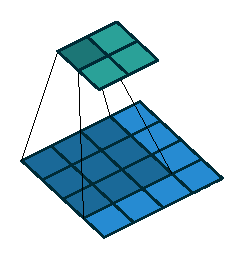
\includegraphics[width=\linewidth]{figures/convolutions/no_padding_no_strides_00.pdf}
        \subcaption*{step 01}
    \end{subfigure}\hfill%
    \begin{subfigure}{0.22\linewidth}
        \centering
        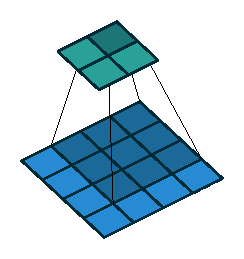
\includegraphics[width=\linewidth]{figures/convolutions/no_padding_no_strides_01.pdf}
        \subcaption*{step 02}
    \end{subfigure}\hfill%
    \begin{subfigure}{0.22\linewidth}
        \centering
        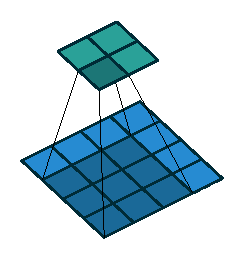
\includegraphics[width=\linewidth]{figures/convolutions/no_padding_no_strides_02.pdf}
        \subcaption*{step 03}
    \end{subfigure}\hfill%
    \begin{subfigure}{0.22\linewidth}
        \centering
        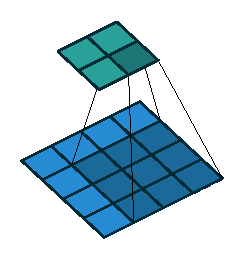
\includegraphics[width=\linewidth]{figures/convolutions/no_padding_no_strides_03.pdf}
        \subcaption*{step 04}
    \end{subfigure}
    \caption{Applying convolutions (by multiplying the input by a kernel) iteratively to different regions (dark blue) of the 2D input (whole blue square). Each iteration gives a numerical value (dark green). The result of all iterations is the green 2D output \cite{dumoulin2016guide}.}
    \label{fig:convolutions}
\end{figure}

\section{Conclusion}
Neural networks are a powerful tool to find the complex relationship between an input and an output (e.g. \acrlong{cm} data and machine degradation). They consist of different layers of interconnected neurons. the connection between each 2 layers is defined by a set of weights, which are multiplied by the values of the previous layer to find the values of the next layer, the process is repeated until the output layer is reached. the predicted output is compared to the actual output obtained from the training data, the weights are adjusted to minimize (using Backpropagation and Gradient Descent) the difference between the predictions and the reality.
